\section{Computational workflow}
\label{sec:computational-workflow}

A \emph{one-pass calculation} fits all supplied observations and checks which requested faces its diagram realizes (Fig.~\ref{fig:computational-workflow}). When neighbor assignments in the supplied pair list are uncertain, some separator predictions may concern pairs that do not share a face in the fitted diagram. Optional refinement repeats the fit on an active subset of these \emph{candidate observations}. Each observation supplies one row of the fitting problem; the \emph{active mask} records which observations enter the current fit. Requested-image face matches determine which candidates remain active, while every original candidate remains available for matching and possible re-entry. The implementation described here is \texttt{pyvoro2} 0.6.3 \cite{Pyvoro2_063}.

\begin{figure}[!tbp]
\centering
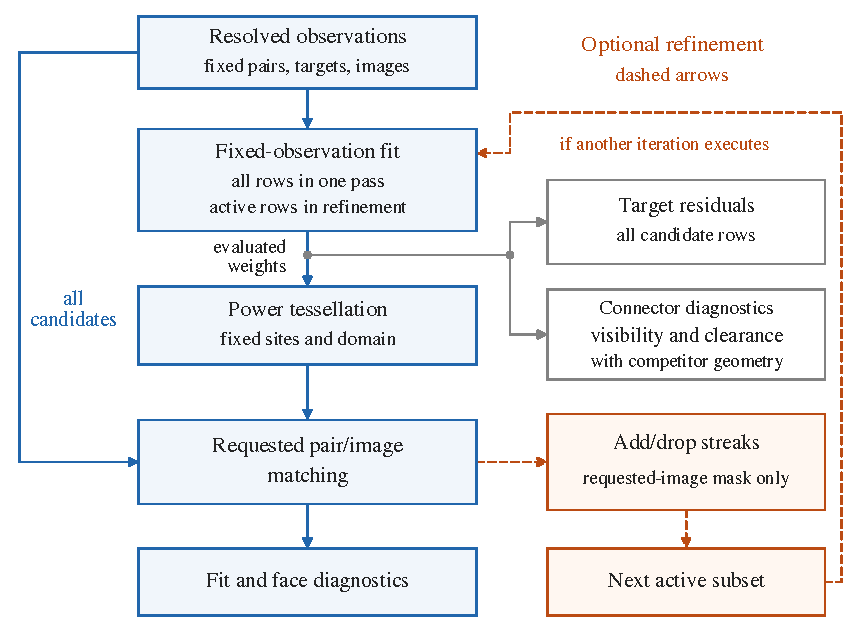
\includegraphics[width=\linewidth]{figures/figure_05_workflow.pdf}
\caption{Data routes for one-pass fitting and optional refinement. Matching receives all resolved candidates; only active rows enter a refined fit. The dashed path updates the active subset using counters of consecutive requested-image realizations or absences. The return to fitting is taken only if another iteration executes. Residuals and connector diagnostics do not drive this update. Sections~\ref{subsec:workflow-active-mask}--\ref{subsec:workflow-output} and~\ref{app:algorithm-implementation} specify alignment, relaxation and finalization.}
\label{fig:computational-workflow}
\end{figure}

\subsection{Resolving observations and fitting a fixed set}
\label{subsec:workflow-fixed-fit}

The inputs are fixed site positions, numerical separator observations, and their assigned fitting weights. A domain is also needed for periodic image resolution or geometric evaluation. Each fitting call uses one measurement convention from Section~2: normalized coordinates or signed distances. An observation retains its ordered pair $(i_r,j_r)$, target $y_r$, and selected image shift $s_r$ in periodic calculations. These choices determine the connector length $d_r$ and affine coefficients $(\alpha_r,\beta_r)$. A supplied periodic shift is part of the observation's identity; when shifts are not supplied, a separate image-selection policy resolves them before fitting. Different shifts for one base pair can label distinct observations while constraining the same weight difference.

For a fixed observation set, the ordinary quadratic fit minimizes the weighted measurement-space residuals of Section~3. With the positive fitting weights assumed there, the implementation solves separately on the observation-graph components using \emph{dense} linear algebra. Since additive component offsets leave the fitted differences unchanged, the solver must choose a representative weight vector on each component. These choices can affect the geometry when several components share a diagram; the version-specific conventions are given in~\ref{app:algorithm-implementation}.

The solver also supports a Huber loss in the original measurement units and hard measurement bounds. A hard restriction applies one common interval or fixed value to every supplied row in those units; this is narrower than the independently indexed restrictions of Section~3.3. Nonquadratic terms or hard restrictions use an iterative solver, and infeasible hard difference bounds are detected by a graph precheck. The Huber threshold is expressed in the selected measurement units, so its equivalent threshold in weight-difference units depends on $\alpha_r$. Predictions are returned as normalized coordinates or signed distances, together with residuals, connectivity warnings, and fitting status. We use the term \emph{fixed-observation fit} to distinguish the rows supplied to the estimator from the faces ultimately realized by the tessellation.

\subsection{Constructing and matching realized faces}
\label{subsec:workflow-realization}

A fitted weight vector $\widehat w$ defines a power diagram but does not guarantee that its observed pairs share actual faces. The three-dimensional backend is Voro++ \cite{Rycroft2009}; two-dimensional calculations use the separately bundled backend exposed by \texttt{pyvoro2.planar} \cite{Pyvoro2_063}. The implementation uses a common shift $C$ such that $\widehat w_i+C\ge0$ and passes radii $r_i=\sqrt{\widehat w_i+C}$. The shift changes none of the power comparisons. Within the chosen two- or three-dimensional domain, the computed cells supply the internal edges or faces that are subsequently matched to the resolved observation rows.

For a periodic observation requesting $(i_r,j_r,s_r)$, the matching step checks that \emph{the specified image shift} occurs among the realized boundaries. The flag \texttt{realized} records a boundary at any shift. An exact requested-image match is marked \texttt{realized\_\allowbreak same\_\allowbreak shift}; if the requested shift is absent but another image is realized, \texttt{realized\_\allowbreak other\_\allowbreak shift} is set. Reversing the pair orientation reverses the shift.

Additional diagnostics flag empty endpoint cells and realized base-site pairs absent from the supplied candidate list, recording the realized shifts of those extra pairs. Boundary length in two dimensions or face area in three dimensions may also be recorded; its image-selection convention is specified in~\ref{app:algorithm-implementation}. Realization here means a boundary reported by the numerical tessellation in the chosen domain.

Requested-image matching examines the actual boundary, whereas the connector tests of Section~4 examine support at a particular point. A realized face can therefore fail connector visibility, as in Fig.~\ref{fig:three-face-cases}(b). Neither property is certified by a small fitting residual.

\subsection{Optional refinement of the observation set}
\label{subsec:workflow-active-mask}

For optional candidate observations, refinement retains a fixed collection of $m$ resolved rows and starts from a Boolean active mask $a^{(0)}\in\{0,1\}^m$, initially all ones unless specified otherwise. At iteration $k$, only rows with $a_r^{(k)}=1$, together with their hard measurement bounds, are supplied to the inner solve. Dropping a row therefore also drops its bound.

For every fit after the first, the weights are aligned component by component with the preceding evaluated weights. Alignment adds a common constant to all weights in each current fitting component, making their mean equal to the preceding mean over the same sites. A relaxation factor $0<\omega\le1$ then blends the aligned fit with the preceding iterate before the diagram is constructed; the initial fit is used without blending. For unregularized fits, alignment preserves the fitting objective while carrying forward component offsets that the pair data do not determine. The optional weight regularizer adds a quadratic penalty for departure from a reference vector. With positive regularization strength, the implementation still aligns the components, which can change the regularized objective; see~\ref{app:algorithm-implementation} for the version-specific regularization and alignment conventions.

The diagram is then evaluated against \emph{every original candidate row}, not only those currently active. For $r=1,\ldots,m$, let
\begin{equation}
v_r^{(k)}=
\begin{cases}
1,&\text{if the requested pair and image shift are realized},\\
0,&\text{otherwise}.
\end{cases}
\label{eq:realized-mask}
\end{equation}
The realized-face mask $v^{(k)}$ drives the update. A present face increments that row's addition streak and resets its removal streak; an absent face does the reverse. For fixed positive integer thresholds $A_{\mathrm{add}}$ and $A_{\mathrm{drop}}$, an inactive row is added after $A_{\mathrm{add}}$ consecutive realized evaluations, while an active row is removed after $A_{\mathrm{drop}}$ consecutive absent evaluations. Until the respective threshold is reached, its membership is unchanged. Thus previously dropped rows can re-enter a later fit, but no candidate pair is created and no supplied image shift is silently changed.

Proposition~\ref{prop:rowwise-hysteresis} shows that $h=\max(A_{\mathrm{add}},A_{\mathrm{drop}})$ consecutive \emph{executed mask updates} with an unchanged realized-face mask suffice for the active mask to agree with it. This conditional bookkeeping result does not show that the realized-face mask becomes stationary or that the coupled fit--tessellation iteration converges.

\subsection{Stopping and interpretation of the returned result}
\label{subsec:workflow-output}

The outer stopping label, the final fitting status, and the geometric diagnostics answer different questions. In particular, a final refit can change the geometry after the last evaluated iteration.

The outer procedure reports \texttt{self\_consistent} when the proposed active mask is unchanged, that mask coincides with the requested-image realization mask, and the change in the evaluated weights has Euclidean norm at most a prescribed tolerance. The label does not by itself certify convergence of the inner numerical solver. Other outcomes include an outer-iteration limit, an infeasible active-row problem, and numerical failure. The \texttt{cycle\_detected} status records a repeated \emph{active mask}; it does not establish a periodic orbit of the weights and streak counters.

After a normal loop stop, the implementation attempts a final, unrelaxed fit on the final active rows. If it returns weights, their component offsets are aligned to the preceding evaluated weights and the resulting diagram is matched again. The final fitting status and weight availability must be checked alongside the outer stopping label: if no weights are returned, the stored realization diagnostics describe the preceding evaluation. The precise stopping and failure conventions are given in~\ref{app:algorithm-implementation}.

When final weights are available, residuals are reported both over all original candidates and over the final active subset. Both root mean square (RMS) summaries are unweighted and expressed in the selected measurement units;~\ref{app:algorithm-implementation} identifies the corresponding output fields. A small residual does not certify a shared face, while an active row need not be realized in the final tessellation.

